%%%%%%%%%%%%%%%%%%%%%%%%%%%%%%%%%%%%%%%%%%%%%%%%%%%%%%%%%%%%%%%%%%%%%%%%%%%%%%%%%%%%%%%%%%%%%%%%%%%%%%%%%%%%%%%%%%%%%%%%%%%%%%%%%%%%%%%%%%%%%%%%%%%%%%%%%%%
% This is just an example/guide for you to refer to when submitting manuscripts to Frontiers, it is not mandatory to use Frontiers .cls files nor frontiers.tex  %
% This will only generate the Manuscript, the final article will be typeset by Frontiers after acceptance.                                                 %
%                                                                                                                                                         %
% When submitting your files, remember to upload this *tex file, the pdf generated with it, the *bib file (if bibliography is not within the *tex) and all the figures.
%%%%%%%%%%%%%%%%%%%%%%%%%%%%%%%%%%%%%%%%%%%%%%%%%%%%%%%%%%%%%%%%%%%%%%%%%%%%%%%%%%%%%%%%%%%%%%%%%%%%%%%%%%%%%%%%%%%%%%%%%%%%%%%%%%%%%%%%%%%%%%%%%%%%%%%%%%%

%%% Version 3.1 Generated 2015/22/05 %%%
%%% You will need to have the following packages installed: datetime, fmtcount, etoolbox, fcprefix, which are normally inlcuded in WinEdt. %%%
%%% In http://www.ctan.org/ you can find the packages and how to install them, if necessary. %%%

\documentclass[english]{frontiers/frontiersSCNS} % for Science, Engineering and Humanities and Social Sciences articles
%\documentclass{frontiersHLTH} % for Health articles
%\documentclass{frontiersFPHY} % for Physics and Applied Mathematics and Statistics articles

\usepackage[mode=buildnew]{standalone}
\usepackage{tikz}
%\setcitestyle{square}
\usepackage{url,lineno,microtype}
\usepackage[toc,nomain,acronym,shortcuts,translate=false]{glossaries}
\usepackage[colorlinks=true,linkcolor=black, citecolor=black!80, urlcolor=black!80]{hyperref}
\usepackage{doi}
\usepackage[onehalfspacing]{setspace}

\def\keyFont{\fontsize{7}{9}\helveticabold }
\def\firstAuthorLast{Esteban {et~al.}} %use et al only if is more than 1 author
\def\Authors{Oscar Esteban\,$^{1,2,*}$, Emmanuel Caruyer\,$^{3}$, Alessandro Daducci\,$^{4}$, Meritxell Bach-Cuadra\,$^{4,5}$,%
Mar\'ia-J. Ledesma-Carbayo\,$^{1,2}$ and Andres Santos\,$^{1,2}$}

\def\Address{%
$^{1}$Biomedical Image Technologies (BIT), ETSI Telecom., Universidad Polit\'ecnica de Madrid, Madrid, Spain \\
$^{2}$Centro de Investigaci\'on Biom\'edica en Red en Bioingenier\'ia, Biomateriales y Nanomedicina (CIBER-BBN), Spain \\
$^{3}$CNRS, IRISA (UMR 6074), VisAGeS research group, Rennes, France \\
$^{4}$Signal Processing Laboratory (LTS5), \'Ecole Polytechnique F\'ed\'erale de Lausanne (EPFL), Lausanne, Switzerland \\
${^5}$Dept. of Radiology, CIBM, University Hospital Center (CHUV) and University of Lausanne (UNIL), Lausanne, Switzerland %
}
% The Corresponding Author should be marked with an asterisk
% Provide the exact contact address (this time including street name and city zip code) and email of the corresponding author
\def\corrAuthor{Oscar Esteban}
\def\corrAddress{Biomedical Image Technologies (BIT), ETSI Telecomunicaci\'on, Av. Complutense 30, C203, E28040 Madrid, Spain}
\def\corrEmail{phd@oscaresteban.es}

% -*- root: main.tex -*-
% @Author: Oscar Esteban
% @Date:   2015-06-16 15:45:32
% @Last Modified by:   Oscar Esteban
% @Last Modified time: 2015-09-15 16:42:48

\newacronym{dmri}{dMRI}{diffusion MRI}
\newacronym{fa}{FA}{fractional anisotropy}
\newacronym{adc}{ADC}{anisotropic diffusion coefficient}
% \newacronym{hcp}{HCP}{Human Connectome Project}
\newacronym{fod}{FOD}{fiber orientation distribution}
\newacronym{fodf}{fODF}{fiber orientation distribution function}
\newacronym{wm}{WM}{white matter}
\newacronym{gm}{GM}{gray matter}
\newacronym{cgm}{cGM}{cortical gray matter}
\newacronym{dgm}{dGM}{deep gray matter}
\newacronym{csf}{CSF}{cerebrospinal fluid}
\newacronym{snr}{SNR}{signal-to-noise ratio}
\newacronym{csd}{CSD}{constrained spherical deconvolution}
\newacronym{cc0}{CC0}{Creative Commons Zero licence}
\newacronym{roc}{ROC}{receiver operating characteristic}
\newacronym{pve}{PVE}{partial volume effect}
\newacronym{cst}{CST}{corticospinal tract}
\newacronym{t1}{T1w}{T1-weighted}

\newglossaryentry{hcp}
{
	name={Human Connectome Project},
	text={HCP},
	first={Human Connectome Project (HCP, \cite{essen_human_2012})},
	long={Human Connectome Project},
	description={Human Connectome Project}
}

\newglossaryentry{bids}%
{
	name={BIDS},
	first={BIDS (Brain Imaging Data Structure, \cite{gorgolewski_brain_2015})},
	long={Brain Imaging Data Structure},
	description={Brain Imaging Data Structure}
}

\newglossaryentry{bedpostx}%
{
	name={BEDPOSTX},
	first={BEDPOSTX (Bayesian Estimation of Diffusion Parameters Obtained using Sampling Techniques modelling crossing --X-- fibres, \cite{jbabdi_modelbased_2012})},
	description={Bayesian Estimation of Diffusion Parameters Obtained using Sampling Techniques modelling crossing --X-- fibres}
}
\newacronym[first={FAST (FMRIB's Automated Segmentation Tool, \cite{zhang_segmentation_2001})}]%
{fast}{FAST}{FMRIB's Automated Segmentation Tool}
\newacronym[first={FIRST (FMRIB's Integrated Registration and Segmentation Tool, \cite{patenaude_bayesian_2011})}]%
{first}{FIRST}{FMRIB's Integrated Registration and Segmentation Tool}

\makeglossaries



\newcommand{\e}[1]{\ensuremath{\;\cdot\,}10\ensuremath{^{#1}}}
\newcommand*\glslines[2][]{\glslink[#1]{#2}{\glsdisp{#2}{\acrlong{#2} --\glsentryshort{#2}--}}}

\begin{document}

\onecolumn
\firstpage{1}

\title[Diffantom]{Diffantom: a whole-brain diffusion MRI phantom derived from a real dataset}

\author[\firstAuthorLast ]{\Authors} %This field will be automatically populated
\address{} %This field will be automatically populated
\correspondance{} %This field will be automatically populated

\extraAuth{}% If there are more than 1 corresponding author, comment this line and uncomment the next one.
%\extraAuth{corresponding Author2 \\ Laboratory X2, Institute X2, Department X2, Organization X2, Street X2, City X2 , State XX2 (only USA, Canada and Australia), Zip Code2, X2 Country X2, email2@uni2.edu}


\maketitle

\linenumbers

\section*{Introduction}
Fiber tracking on \gls*{dmri} data has become an important application for the in-vivo investigation
  of the structural configuration of fiber bundles at the macro-scale.
Tractography is fundamental to gain information about \gls*{wm} morphology in many clinical routines
  like neurosurgical planning \citep{golby_interactive_2011}, post-surgery evaluations \citep{toda_utility_2014},
  and the study of neurological diseases as in \citep{chua_diffusion_2008} addressing multiple sclerosis and
  Alzheimer's disease.
Tractography is also applied in research for the analysis of structural brain networks using graph theory.
These analyses have been successfully applied in the definition of the unique subject-wise patterns of connectivity
  \citep{sporns_human_2005}, the assessment of neurological diseases \citep{griffa_structural_2013}, and in the
  study of the link between structural and functional connectivity \citep{messe_predicting_2015}.
However, the development of the field is limited by the lack of a gold standard to test and compare the
  wide range of methodologies available for processing and analyzing \gls*{dmri}.

Large efforts have been devoted to the development of physical phantoms
  \citep{lin_validation_2001,campbell_flowbased_2005,perrin_validation_2005,fieremans_simulation_2008,tournier_resolving_2008}.
\cite{cote_tractometer_2013} conducted a thorough review of tractography methodologies using the
  so-called \emph{FiberCup} phantom \citep{poupon_new_2008,fillard_quantitative_2011}.
These phantoms are appropriate to evaluate the angular resolution in fiber crossings and accuracy of
  direction-independent scalar parameters in very simplistic geometries.
Digital simulations are increasingly popular because the complexity of whole-brain tractography
  can not be accounted for with current materials and proposed methodologies to build physical phantoms.
Early digital phantoms also started with simulation of simple geometries
  \citep{basser_in_2000,goessl_fiber_2002,tournier_limitations_2002,leemans_mathematical_2005}
  to evaluate resolution of fiber crossings.
These tools generally implemented the multi-tensor model \citep{alexander_analysis_2001,tuch_high_2002}
  to simulate fiber crossing, fanning, kissing, etc.
\cite{close_software_2009} presented the \emph{Numerical Fibre Generator}, a software to simulate
  spherical shapes filled with digital fiber-tracts.
\cite{caruyer_phantomas_2014} proposed \emph{Phantomas} to simulate any kind of analytic geometry
  inside a sphere.
\emph{Phantomas} models diffusion by a restricted and a hindered compartment, similar to
  \citep{assaf_composite_2005}.
\cite{wilkins_fiber_2014} proposed a whole-brain simulated phantom derived from voxel-wise orientation
  of fibers averaged from real \gls*{dmri} scans and the multi-tensor model with a compartment of
  isotropic diffusion.
\cite{neher_fiberfox_2014} proposed \emph{FiberFox}, a visualization software to develop
  complex geometries and their analytical description.
Once the geometries are obtained, the software generates the corresponding \gls*{dmri} signal with a
  methodology very close to that implemented in \emph{Phantomas}.
An interesting outcome of \emph{FiberFox} is the phantom dataset\footnote{Available at
  \url{http://www.tractometer.org/ismrm_2015_challenge/}} created for the Tractography
  Challenge held in ISMRM 2015.
This dataset was derived from the tractography extracted in one \gls*{hcp} dataset.
In the tractogram, 25 fiber bundles of interest were manually segmented by experts.
Using \emph{FiberFox}, the segmentation of each bundle was mapped to an analytical
  description and finally simulated the signal.

\emph{Diffantom} is originally designed for the investigation of susceptibility-derived distortions, a
  typical artifact that produces geometrical warping in certain regions of \gls*{dmri} datasets.
In \citep{esteban_simulationbased_2014} we addressed this phenomenon and concluded that the connectivity
  matrix of \emph{Phantomas} was not dense enough to evaluate the integration of correction methods
  in pipelines for the connectome extraction.
In this report we present \emph{diffantom}, an \emph{in-silico} dataset to assess pipelines for tractography
  and connectome extraction using real data as source of whole-brain microstructural information.
\emph{Diffantom} is inspired by the work of \cite{wilkins_fiber_2014}, with two principal novelties.
First, since we use a dataset from the \gls*{hcp} as input, data are corrected for the most relevant distortions.
\cite{wilkins_fiber_2014} explicitly state that their original data were not subjected to certain distortion
  corrections, and thus, generated data are affected correspondingly.
The second improvement is a more advanced signal model to generate the phantom using the hindered and restricted
  diffusion model of \emph{Phantomas} \citep{caruyer_phantomas_2014}.


\section*{Data description}

\noindent\textbf{\textit{Microstructural model\textcolon}\label{sec:data_model}} %
The simulation process relies on a microstructural model derived from real data.
On one hand, the software requires up to five fraction maps $\{T_{1\,\cdots\,5}\}$ of
  free- and hindered- diffusion (see \autoref{fig:figure1}, box A).
These compartments will be derived from the macroscopic structure of tissues within the brain,
  specified in the following order~%
\footnote{Corresponding to the \emph{5TT format} established with the latest version 3.0
  of \emph{MRTrix} \citep{tournier_mrtrix_2012}}:
\gls*{cgm}, \gls*{dgm}, \gls*{wm}, \gls*{csf}, and abnormal tissue~%
\footnote{Since here we simulate healthy subjects, the last fraction map is empty and can be omitted}.
On the other hand, the restricted-diffusion compartments are specified by up to three volume fractions $\{F_{1\,\cdots\,3}\}$
  of three single fiber populations per voxel along with their corresponding direction maps $\{V_{1\,\cdots\,3}\}$.

The process to obtain the microstructural model can be described like follows:
1) The fiber orientation maps $\{V_{1\,\cdots\,3}\}$ and their corresponding fiber-fraction maps are
  obtained using the ball-and-stick model for multi-shell data of BEDPOSTX \citep{jbabdi_modelbased_2012}
  on the \gls*{dmri} data of a certain \gls*{hcp} subject.
2) A \gls*{fa} map is obtained after fitting a tensor model with \emph{MRTrix}.
3) The original fiber-fractions and the \gls*{fa} map are smoothed with a non-local means filter included
  in \emph{dipy} \citep{garyfallis_dipy_2011}.
4) The macrostructural 5TT map is extracted from the \acrlong*{t1} image of the subject, using \emph{MRTrix} tools.
5) The objects obtained in the previous steps are combined as described in the \nameref{sec:appendix} to generate the
  microstructural model, presented in \autoref{fig:figure1}-A.

\noindent\textbf{\textit{Diffusion signal generation\textcolon}\label{sec:data_dwi}} %
Once a microstructural model of the volume has been synthesized, a map of \glspl{fod} is computed using spherical
  convolution of the single fiber response and the fiber orientation maps $\{V_{1\,\cdots\,3}\}$, weighted by the
  corresponding fiber-fractions $\{F_{1\,\cdots\,3}\}$.
A close-up showing how the \glspl{fod} map looks is presented in \autoref{fig:figure1}.
The single fiber response is a Gaussian diffusion tensor with axial symmetry and eigenvalues $\lambda_1=$ 2.2\e{-3}
  and $\lambda_{2,3}=$ 0.2\e{-3} [mm$^2$s$^{-1}$].
The resulting \glspl{fod} map is then combined with the isotropic compartments corresponding to $\{T_{1\,\cdots\,5}\}$
  before generating the signal using \emph{Phantomas} \citep{caruyer_phantomas_2014}.
By default, diffusion data are generated using a scheme of 100 directions distributed in one shell with uniform
  coverage \citep{caruyer_design_2013}.
Custom one- or multi-shell schemes can be generated supplying the tables of corresponding $b$-vectors and $b$-values.
Rician noise is also included in \emph{Phantomas}, and can be set by the user.
The default value for \gls*{snr} is preset to 90.0.
\Gls*{csf} was simulated with a unique compartment with isotropic diffusivity $D_{CSF}$ of 3.0\e{-3} [mm$^2$s$^{-1}$].
Conversely, \Gls*{wm} and \gls*{gm} included one isotropic compartment with $D_{WM} =$ 2.0\e{-4}, $D_{cGM} =$ 7.0\e{-4}
  and $D_{dGM} =$ 9.0\e{-4}, respectively [mm$^2$s$^{-1}$].
All these values for diffusivity (and the corresponding to the single-fiber response) can be modified by the user with
  custom settings.


\noindent\textbf{\textit{Implementation and reproducibility\textcolon}\label{sec:data_workflow}} %
We also provide the full software stack used to generate \emph{diffantoms}, so that users can
  regenerate similar datasets with different parameters.
This workflow, presented in \autoref{fig:figure1}, is implemented using
  \emph{nipype} \citep{gorgolewski_nipype_2011} to ensure reproducibility and usability.

\noindent\textbf{\textit{Interpretation and recommended uses\textcolon}\label{sec:data_use}} %
To illustrate the features of the \emph{diffantom}, the example dataset underwent a simplified
  connectivity pipeline including \gls*{csd} and probabilistic tractography from
  \emph{MRTrix} \citep{tournier_mrtrix_2012}.
\Gls*{csd} was configured with up to 8 spherical harmonics, and tractography with 1.6$\times$10$^\text{6}$
  seed points evenly distributed across a dilated mask of the \gls*{wm} tissue.
\autoref{fig:figure2}, box B1 shows the result of the tractography obtained with such pipeline.
Finally, we applied \emph{tract querier} \citep{wassermann_on_2013} on segmenting important fiber bundles such
  as the \gls*{cst} and the forceps minor (see \autoref{fig:figure2}, box B2).
Particularly, due to its location nearby the orbitofrontal lobe, the forceps minor is generally affected by
  susceptibility distortions.

Since the gradient scheme can be set by the user, \emph{diffantom} can be seen as a mean to translate the so-called
  \emph{b-matrix} of the \gls*{hcp} to any target scheme.
A second recommended use case of the simulation workflow is its integration in assessment frameworks
  (\autoref{fig:figure2}, box A) for the unit testing of algorithms, the integration tests of
  modules in workflows and the full validation of pipelines.
The \emph{diffantom} enables the following evaluations of connectivity pipelines:
\begin{itemize}
  \item Studies on the impact of different diffusion sampling schemes on the local micro-structure
  model of choice and on the subsequent global tractography outcome.
  \item Assessment of sensitivity and robustness to imaging artifacts (noise, \acrlong{pve} and \glslines{csf} contamination,
    susceptibility-derived warping, Eddy-currents-derived distortions, etc.) at both local and global levels.
  \item Characterizing the \acrfull*{roc} of connectivity pipelines.
  \item Generation of synthetic connectivity networks to test graph theory analyses.
  \item Simulation of pathological brains (e.g. tumors as in \cite{kaus_simulation_2000}).
\end{itemize}

\section*{Discussion and conclusion}
\noindent\textbf{\textit{Discussion\textcolon}}\label{sec:discussion} %
Whole-brain, realistic \gls*{dmri} phantoms are necessary in the developing field of structural
  connectomics.
The \emph{diffantom} is a derivative of \citep{wilkins_fiber_2014} in terms of methodology for
  simulation with two major advances: the correctness of the \emph{minimally preprocessed} data
  \citep{glasser_minimal_2013} released within the \gls*{hcp}, and a more realistic diffusion
  model.
A possible competitor to \emph{diffantom} is the phantom generated for the Tractography Challenge in
  ISMRM 2015.
Similarly to \emph{diffantom}, they organizers used a \gls*{hcp} subject as source of structural information.
While this phantom is designed for the bundle-wise evaluation of tractography (with scores such as geometrical coverage,
  valid connections, invalid connections, missed connections, etc. \citep{cote_tractometer_2013}),
  \emph{diffantom} is intended for the connectome-wise evaluation of results, yielding tractography with
  a large number of bundles.
Therefore, \emph{diffantom} and \emph{FiberFox} are complementary as the hypotheses that can be investigated are different.
Moreover, \emph{diffantom} does not require costly manual segmentation of bundles, highly demanding in terms of physiology
  expertise and operation time.
This facilitates the use of \emph{diffantom} as a factory of whole-brain diffusion phantoms.

\noindent\textbf{\textit{Conclusion\textcolon}}\label{sec:conclusion} %
\emph{Diffantom} is a digital phantom generated from a dataset belonging to the \acrlong*{hcp}, and the software factory to
  reproduce it.
The first \emph{diffantom} is presented here to be openly and freely distributed along with the necessary resources to
  generate new \emph{diffantoms}.
We encourage the neuroimage community to contribute with their own \emph{diffantoms} and share them openly.


\section*{Data Sharing}
The first \emph{diffantom} is available under the \gls*{cc0} in {\color{red} (dryad?)}.
The associated software to ``\emph{diffantomize}'' real \gls*{dmri} data is available at \url{https://github.com/oesteban/diffantom}
  under an MIT license.
\emph{Phantomas} is available in \url{https://github.com/ecaruyer/Phantomas} under the revised-BSD license.

\section*{Disclosure/Conflict-of-Interest Statement}

The authors declare that the research was conducted in the absence of any commercial or financial relationships that could be construed as a potential conflict of interest.

\section*{Author Contributions}
All the authors contributed to this study.
OE designed the data generation procedure, implemented the processing pipelines and generated the example dataset.
EC implemented \emph{Phantomas} \citep{caruyer_phantomas_2014}, helped integrate the project with the simulation routines.
OE, EC, AD thoroughly discussed and framed the aptness of the data in the community.
AD, MBC, MJLC, and AS interpreted the resulting datasets.
MBC, MJLC, and AS advised on all aspects of the study.


\section*{Acknowledgments}
We thank Gert Wollny for his revision of this work.
\textit{Funding\textcolon}
This study was supported by the Spanish Ministry of Science and Innovation
  (projects TEC-2013-48251-C2-2-R and INNPACTO XIORT), Comunidad de Madrid (TOPUS) and
  European Regional Development Funds, the Center for Biomedical Imaging
  (CIBM) of the Geneva and Lausanne Universities and the EPFL, as well as the
  Leenaards and Louis Jeantet Foundations.

\nolinenumbers
\bibliographystyle{frontiers/frontiersinSCNS_ENG_HUMS}
%\bibliographystyle{frontiersinHLTH&FPHY} % for Health and Physics articles
\bibliography{Remote}

%%% Upload the *bib file along with the *tex file and PDF on submission if the bibliography is not in the main *tex file

\glsresetall
\linenumbers
\section*{Appendix}\label{sec:appendix}
Let $\{T'_{1\,\cdots\,5}\}$ be the set of original fractions maps obtained with \texttt{act\_anat\_prepare\_fsl}, a
  tool in \emph{MRTrix} that combines FAST \citep{zhang_segmentation_2001} and FIRST \citep{patenaude_bayesian_2011}
  to generate the macrostructural 5TT map.
FA denotes the \gls*{fa} map obtained from the original \gls*{dmri} data, and $\{V_{1\,\cdots\,3}, F'_{1\,\cdots\,3}\}$ the direction
  maps $V_i$ of restricted diffusion by fibers with their estimated volume fractions $F'_i$ calculated with BEDPOSTX.
The final $\{T_{1\,\cdots\,5}\}$ maps of isotropic fractions are computed as follows:

  \begin{align*}
  T_1 &= (1.0-f_{cgm}) \cdot T'_1 \\
  T_2 &= (1.0-f_{dgm}) \cdot T'_2 \\
  T_3 &= (1.0-f_{wm}) \cdot T'_3 \\
  T_4 &= T'_4 \\
  T_5 &= 0.0
  \end{align*}
where $f_{\{cgm, dgm, wm\}}$ are the fractions of restricted diffusion for each tissue.
\cite{sepehrband_brain_2015} found out that the fiber fraction ranges across the corpus
  callosum from the 70$\pm$8\% in its body to an upper bound of 80$\pm$11\% in the splenium.
Therefore, we choose $f_{wm} =$ 80\% as default fraction of restricted diffusion in the
  \gls*{wm}.
To our knowledge, restricted diffusion fractions have been studied only for \gls*{wm}.
Therefore, we set $f_{cgm} =$ 25\% and $f_{dgm} =$ 50\% as they yield plausible \gls*{fa}
  and \gls*{adc} maps, assessed visually.
The final $\{F_{1\,\cdots\,3}\}$ maps are computed as follows:

\begin{align*}
F_1 &= f_{wm} \cdot T_2 \cdot \text{FA} + w_{f1} (f_{cgm} \cdot T_1 + f_{dgm} \cdot T_2) \\
F_2 &= f_{wm} \cdot T_2 - (F_1 + F_3) + w_{f2} (f_{cgm} \cdot T_1 + f_{dgm} \cdot T_2) \\
F_3 &= f_{wm} \cdot F'_3 + w_{f3} (f_{cgm} \cdot T_1 + f_{dgm} \cdot T_2)
\end{align*}
where $w_{\{f1, f2, f3\}}$ are the contributions of the \gls*{gm} compartments to each fiber population.
By default: $w_{f1} = $ 48\%, $w_{f2} = $ 37\%, $w_{f3} = $ 15\%.
Finally, the resulting maps are normalized to fulfill $\sum_i T_i + \sum_i F_i = 1.0$.

\newpage
\section*{Figures}

\begin{figure}[h!]
\begin{center}
\includestandalone[width=\linewidth]{figure01}
\end{center}
\textbf{\refstepcounter{figure}\label{fig:figure1} Figure \arabic{figure}. }%
{\textbf{Generation of \emph{diffantoms}:} First, a microstructural model is generated as described
  in the \nameref{sec:data_generation} subsection.
Please note the piece-wise linear function of the color scale to enable visibility of small volume fractions.
This microstructural model is fed into a simulation block that generates the final \gls*{dmri} dataset
  as described in the second block.
}
\end{figure}

\begin{figure}[h!]
\begin{center}
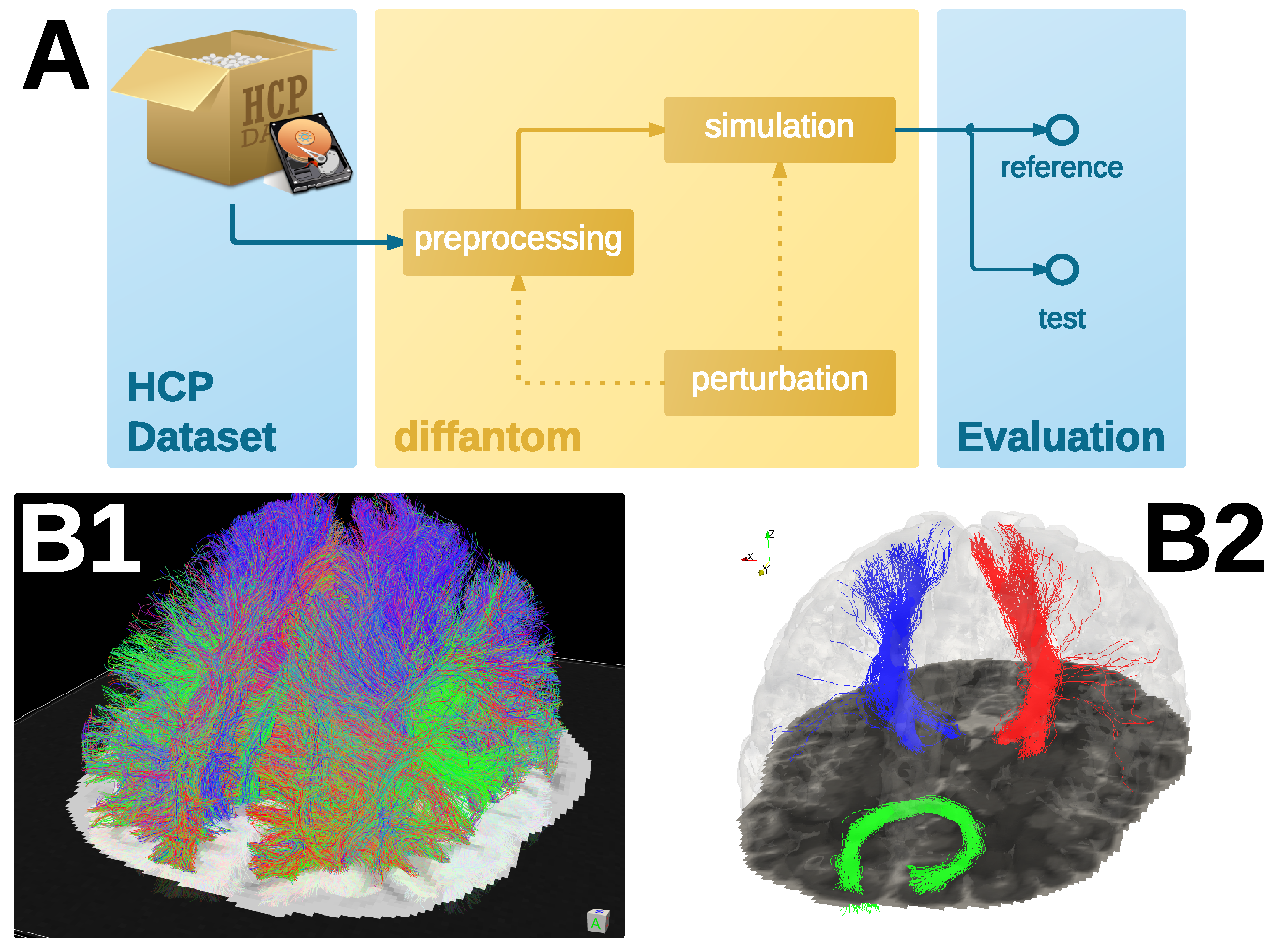
\includegraphics[width=\linewidth]{figures/figure02}
\end{center}
\textbf{\refstepcounter{figure}\label{fig:figure2} Figure \arabic{figure}. }%
{\textbf{A. Recommended use of \emph{diffantom}}.
The dataset can be used to test algorithms and pipelines against a perturbation that is
  introduced in \emph{diffantom}.
Perturbations can model typical artifacts found in \gls*{dmri} datasets or pathological conditions
  such as a tumor.
\textbf{B1. Tractogram of fibers crossing slice 56 of the \emph{diffantom}} represented over that corresponding
  slice of the \emph{b0} volume. \textbf{B2. Segmentation of some fiber bundles}: the right \gls*{cst} is
  represented in blue color, the left \gls*{cst} in red, and the forceps minor in green.
  The box includes the slice 56 of the \emph{b0} and the pial surface is represented with a light gray shadow.
}
\end{figure}

\end{document}
